\chapter{Void methods}

So far we've only written short programs that have a single class with a \java{main} method.
In this chapter, we'll show you how to organize longer programs into multiple methods and classes.
%We will also take a look at separate compilation.

\index{method}

At a conceptual level, a {\bf method} represents a {\em function} or {\em procedure}.
Functions perform a computation and return a result.
For example, \java{Math.sqrt(25)} returns the value \java{5.0}.
Procedures simply carry out a sequence of actions without returning a result.
We refer to them as \java{void} methods.


\section{Math methods}

\index{Math class}
\index{class!Math}
\index{expression}
\index{argument}

In mathematics, you have probably seen functions like $\sin$ and $\log$, and you have learned to evaluate expressions like $\sin(\pi/2)$ and $\log(1/x)$.
First, you evaluate the expression in parentheses, which is called the {\bf argument} of the function.
Then you can evaluate the function itself, either by looking it up in a table or by performing various computations.

This process can be applied repeatedly to evaluate more complex expressions like $\log(1/\sin(\pi/2))$.
First we evaluate the argument of the innermost function, then evaluate the function itself, and so on.

Java provides a \java{Math} class that performs the most common mathematical operations.
%These functions are called {\bf methods}.
The math methods are invoked using a syntax that is similar to the \java{print} statements we have already seen:

\begin{code}
    double root = Math.sqrt(17.0);
    double angle = 1.5;
    double height = Math.sin(angle);
\end{code}

The first line sets \java{root} to the square root of 17.
The third line finds the sine of the value of \java{angle}.

\index{degrees}
\index{radians}

Java assumes the values you use with trigonometric functions (\java{sin}, \java{cos}, \java{tan}) are in {\em radians}.
To convert from degrees to radians, you can divide by 360 and multiply by $2 \pi$.
Conveniently, Java provides the constant \java{Math.PI}:

\begin{code}
    double degrees = 90;
    double angle = degrees * 2 * Math.PI / 360.0;
\end{code}

Notice that \java{PI} is in all capital letters.
Java does not recognize \java{Pi}, \java{pi}, or \java{pie}.

\index{type!long}

Another useful method in the \java{Math} class is \java{round}, which rounds a floating-point value to the nearest integer and returns a \java{long}.
In Java, \java{int} values are 32 bits and \java{long} values are 64 bits.
As a result, \java{long} variables can represent much larger (and smaller) integers.

\begin{code}
    long x = Math.round(Math.PI * 20.0);
\end{code}

In this example the multiplication happens first, before the method is invoked.
The result is 63 (rounded up from 62.8319).

\subsection{Composition revisited}

\index{composition}
\index{expression}

Just as with mathematical functions, Java methods can be {\bf composed}.
That means you can use one expression as part of another.
For example, you can use any expression as an argument to a method:

\begin{code}
    double x = Math.cos(angle + Math.PI / 2);
\end{code}

This statement takes the value \java{Math.PI}, divides it by two, and then adds the result to the value of the variable \java{angle}.
The sum is then passed as an argument to \java{cos}.

Note that \java{PI} is the name of a variable, not a method.
A variable is a {\em location of data}, whereas a method is a {\em location of code}.
In Java, methods always have parentheses, even if they have no arguments like \java{System.out.println()}.

You can also take the result of one method and pass it as an argument to another method:

\begin{code}
    double x = Math.exp(Math.log(10.0));
\end{code}

In Java, the \java{log} method always uses base $e$.
So this statement finds the log base $e$ of 10, and then raises $e$ to that power.
The result gets assigned to \java{x}.
Do you know what it is without reaching for a calculator?

\section{Adding new methods}
\label{adding_methods}

\index{method!definition}
\index{main}
\index{method!main}

In addition to calling methods from Java libraries, you can also define your own methods.
%We have already seen one method definition: {\tt main}.
For \java{void} methods, the syntax is similar to \java{main}:

\begin{code}
    public static void NAME(PARAMETERS) {
        STATEMENTS
    }
\end{code}

You can use any name you want for your method, except that you can't call it \java{main} or any of the Java keywords.
By convention, methods start with a lower case letter and use ``camelCase,'' which is a cute name for {\tt jammingWordsTogetherLikeThis}.

\index{invoke}

The list of parameters specifies what values, if any, you have to provide in order to use (or {\bf invoke}) the new method.

The parameter for \java{main} is \java{String[] args}, which means that whoever invokes \java{main} must provide an array of Strings (we'll get to arrays in a later chapter).
The first methods we are going to write have no parameters, so the syntax looks like this:

\begin{code}
    public static void newLine() {
        System.out.println();
    }
\end{code}

This method is named {\tt newLine}, and the empty parentheses mean that it takes no parameters.
It contains one statement, which prints a blank line.
%Printing a {\tt String} with no letters in it may not seem all that useful, but {\tt println} skips to the next line after it prints, so this statement skips to the next line.
In {\tt main}, we can invoke this new method the same way we call library methods:

\begin{code}
    public static void main(String[] args) {
        System.out.println("First line.");
        newLine();
        System.out.println("Second line.");
    }
\end{code}

The output of this program is:

\begin{stdout}
First line.

Second line.
\end{stdout}

Notice the extra space between the lines.
If we wanted more space between them, we could invoke the same method repeatedly:

\begin{code}
    public static void main(String[] args) {
        System.out.println("First line.");
        newLine();
        newLine();
        newLine();
        System.out.println("Second line.");
    }
\end{code}

Or we could even write a new method that prints three blank lines:

\begin{code}
    public static void threeLine() {
        newLine();
        newLine();
        newLine();
    }

    public static void main(String[] args) {
        System.out.println("First line.");
        threeLine();
        System.out.println("Second line.");
    }
\end{code}

Notice that you can invoke the same method more than once.
You can also have one method invoke another method.
In this example, \java{main} invokes \java{threeLine}, and \java{threeLine} invokes \java{newLine}.

%In {\tt threeLine} I wrote three statements all on the same line, which is syntactically legal (remember that spaces and new lines usually don't change the meaning of a program).
%It is usually a good idea to put each statement on its own line, but I sometimes break that rule.

You might wonder why it is worth the trouble to create all these new methods.
There are many reasons, but this example demonstrates a few of them:

\begin{enumerate}

\item
%Creating a new method gives you an opportunity to give a name to a group of statements.
Methods simplify a program by hiding complex computations behind a single statement, and by using English words in place of arcane code.
%Which is clearer, {\tt newLine} or {\tt System.out.println()}?

\item Creating a new method can make a program smaller by eliminating repetitive code.
For example, to print nine consecutive new lines, you could invoke \java{threeLine} three times.

\item A common problem-solving technique is to break things down into sub-problems.
Methods allow you to focus on each sub-problem in isolation, and then compose them into the final solution.

\end{enumerate}

%In Section~\ref{methods} we will come back to this question and list some additional benefits of dividing programs into methods.

%Perhaps most importantly, organizing your code into multiple methods allows you to test individual parts of your program separately.


\section{Classes and methods}

\index{class}
\index{method}

Pulling together the code fragments from the previous section, the program looks like this:

\begin{code}
public class NewLine {

    public static void newLine() {
        System.out.println();
    }

    public static void threeLine() {
        newLine();
        newLine();
        newLine();
    }

    public static void main(String[] args) {
        System.out.println("First line.");
        threeLine();
        System.out.println("Second line.");
    }

}
\end{code}

The first line is the class definition.
Class names should be capitalized; this convention helps readers tell the difference between classes and methods in your source code.
%A {\bf class} is a collection of related methods.
The \java{NewLine} class contains three methods named \java{newLine}, \java{threeLine}, and \java{main}.
Since Java is a case-sensitive language, the names \java{NewLine} and \java{newLine} are considered different tokens.

The other class we've seen is the \java{Math} class.
It contains methods named \java{sqrt}, \java{sin}, and many others.
(If you haven't yet already, take a look at the documentation for \java{Math}.)
When we invoke a method in another class, we have to specify both the name of the class and the name of the method.
%That's why the syntax is slightly different for Java methods and the methods we write:

\begin{code}
    Math.pow(2.0, 10.0);
    newLine();
\end{code}

The first statement invokes the \java{pow} method in the \java{Math} class, which raises the first argument to the power of the second argument.
The second statement invokes the \java{newLine} method, which Java assumes is in the current class we are writing (i.e., {\tt NewLine}).

If you try to invoke a method from the wrong class, the compiler will give an error.
For example, if you type:

\begin{code}
    pow(2.0, 10.0);
\end{code}

The compiler will say ``cannot find symbol'' which means ``I can't find a method named \java{pow} in the class \java{NewLine}.''
If you have seen this message before, you might have wondered why it was looking for \java{pow} in your class instead of the \java{Math} class.
Now you know.


\section{Programs with multiple methods}

\index{order of execution}

When you look at a class definition that contains several methods, it is tempting to read it from top to bottom.
But that is likely to be confusing, because that is not the {\bf order of execution} of the program.

Execution always begins at the first statement of \java{main}, regardless of where it is in the source file.
In the previous example, we deliberately put \java{main} at the bottom of the program.
Statements are executed one at a time, in order, until you reach a method invocation.
Think of method invocations as a detour in the flow of execution.
Instead of going to the next statement, you go to the first line of the invoked method, execute all the statements there, and then come back and pick up again where you left off.

That sounds simple enough, except that you have to remember that one method can invoke another one.
Thus, while we are in the middle of \java{main}, we might have to go off and execute the statements in \java{threeLine}.
But while we are executing \java{threeLine}, we get interrupted multiple times to go off and execute \java{newLine}.

For its part, \java{newLine} invokes \java{println}, which causes yet another detour.
Fortunately, Java is adept at keeping track of where it is.
So when \java{println} completes, it picks up where it left off in \java{newLine}, and then gets back to \java{threeLine}, and then finally gets back to \java{main} so the program can terminate.

Technically, the program does not terminate at the end of \java{main}.
Instead, execution picks up where it left off in the program that invoked \java{main}, which is the Java interpreter.
The interpreter takes care of things like deleting windows and general cleanup, and {\em then} the program terminates.

%What's the moral of this sordid tale?
%When you read a program, don't read from top to bottom.
%Instead, follow the flow of execution.


\section{Parameters and arguments}

\index{parameter}
\index{argument}

Some of the methods we have used require arguments, which are values that you provide when you invoke the method.
For example, to find the sine of a number, you have to provide the number.
So \java{sin} takes a \java{double} as an argument.
To print a message, you have to provide the string.
So \java{println} takes a \java{String} as an argument.
Some methods take more than one argument.
For example, \java{Math.pow} takes two \java{double} values: the base and the exponent.

When you use a method, you simply provide the arguments.
But when you write a method, you must specify a list of parameters.
A {\bf parameter} is a {\em variable} that stores an argument.
The parameter list indicates what arguments are required.
For example, \java{printTwice} specifies a single parameter \java{s} that has type \java{String}.
%I called it {\tt s} to suggest that it is a {\tt String}, but I could have given it any legal variable name.
In order to invoke \java{printTwice}, we have to provide a single argument with type \java{String}.

\begin{code}
    public static void printTwice(String s) {
        System.out.println(s);
        System.out.println(s);
    }
\end{code}

When you invoke a method, the arguments get assigned to the parameters.
In this example, the argument \java{"Don't make me say this twice!"} is assigned to the parameter \java{s}.

\begin{code}
    printTwice("Don't make me say this twice!");
\end{code}

\index{parameter passing}

This process is called {\bf parameter passing} because the value gets passed from outside the method to the inside.
An argument can be any kind of expression, so if you have a {\tt String} variable, you can use it as an argument:

\begin{code}
    String argument = "Never say never.";
    printTwice(argument);
\end{code}

The value you provide as an argument must have the same type as the parameter.
For example, if you try:

\begin{code}
    printTwice(17);
\end{code}

You will get the compiler error ``cannot find symbol,'' which isn't very helpful.
Java is looking for a method named \java{printTwice} that can take an integer.
Since there isn't one in the current class, Java can't find such a ``symbol.''

On the other hand, the same automatic conversion rules apply to parameter passing as for assignment.
For example, \java{Math.sqrt} requires a \java{double} value.
If you run \java{Math.sqrt(25)}, the value \java{25} is automatically converted to \java{25.0}.

%\java{System.out.println} can accept any type as an argument.
%But generally speaking, that is an exception; most methods are not so accommodating.


\section{Stack diagrams and scope}
\label{stack}

\index{stack diagram}
\index{diagram!stack}

Parameters and other variables only exist inside their own methods.
Within the confines of \java{main}, there is no such thing as \java{s}.
If you try to use it there, the compiler will complain.
Similarly, inside \java{printTwice} there is no such thing as \java{argument}.
That variable belongs to the \java{main} method.

One way to keep track of where each variable is defined is to draw a {\bf stack diagram}.
The stack diagram for the previous example looks like this:

\begin{center}
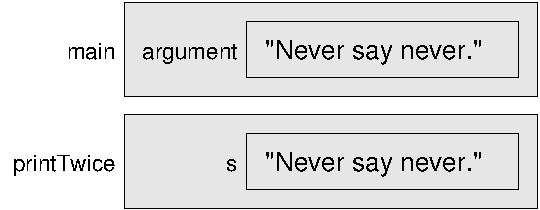
\includegraphics{stack.pdf}
\end{center}

\index{frame}

For each method there is a gray box called a {\bf frame} that contains the method's parameters and variables.
The name of the method appears outside the frame.
As before, the value of each variable is drawn inside a box with the name of the variable beside it.

Stack diagrams help you to visualize the {\bf scope} of a variable, which is the area of a program where a variable exists.
It's possible to reuse the same variable name in two different methods.
But since they each have a different scope, they are not stored in the same memory location.


\section{Tracing code using a debugger}

\index{debugger}

Keeping track of variables and methods on paper is a useful skill, and you should practice drawing stack diagrams.
Another way to visualize the scope of variables and the flow of execution is to use a {\bf debugger}.
The overall process is the same, regardless which development environment you use:

\index{breakpoint}

\begin{enumerate}
\item Set {\bf breakpoints} on lines where you want the program to pause.
\item Step through the code one line at a time and watch what it does.
\item Check the current values of variables and see when they change.
\end{enumerate}

For example, open any program in DrJava and move the cursor to the first line of \java{main}.
Press Ctrl+B to toggle a breakpoint on the current line; it should now be highlighted in red.
Press Ctrl+Shift+D to turn on Debug Mode; a new pane should appear at the bottom of the window.
(These commands are available from the {\em Debugger} menu, in case you forget the shortcut keys.)

\index{call stack}

At this point when you run your program, the execution will pause on the first breakpoint.
The debug pane shows the {\bf call stack}, with the current method on top of the stack.
You might be surprised to see how many methods were called before the \java{main} method!
To the right are several buttons that allow you to step through the code at your own pace.
You can also press ``Automatic Trace'' to watch DrJava run your code one line at a time.

\begin{figure}[!h]
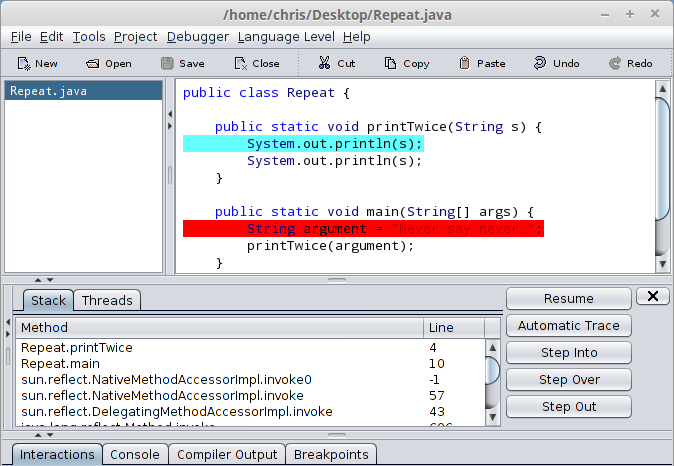
\includegraphics[width=\textwidth]{debugger.png}
\caption{Screenshot of the DrJava debugger.
Execution is currently paused on the first line of \java{printTwice}.
There is a breakpoint on the first line of \java{main}.}
\end{figure}

When the program is paused, you can examine (or even change) the value of any variable using the Interactions Pane.
This feature allows you to verify your assumptions about how data is passed from one method to another, as well as how the resulting values are computed and returned.

Using a debugger is like having the computer proofread your code out loud.
You may think the code will do one thing, and then the debugger shows it doing something else.
At that moment, you gain insight about what may be wrong with the code.

You can edit your code while debugging it, but the changes won't take effect until after you compile.
%The debugger may get out of sync if you add or delete multiple lines of code while the program is paused.


\section{Methods with multiple parameters}
\label{time}

\index{parameter!multiple}
\index{method!multiple parameter}
\index{class!Time}

The syntax for declaring and invoking methods with multiple parameters is a common source of confusion.
For one, you have to declare the type of every parameter separately.

\begin{code}
    public static void printTime(int hour, int minute) {
        System.out.print(hour);
        System.out.print(":");
        System.out.println(minute);
    }
\end{code}

It might be tempting to write \java{int hour, minute} but that format is only legal for variable declarations, not parameter lists.

Another common source of confusion is that you do not have to declare the types of arguments.
The following is incorrect:

\begin{code}
    int hour = 11;
    int minute = 59;
    printTime(int hour, int minute);  // syntax error
\end{code}

In this case, Java can already tell the type of \java{hour} and \java{minute} by looking at their declarations.
It is unnecessary (and therefore not allowed) to include the type when you pass them as arguments.
The correct syntax is:

\begin{code}
    printTime(hour, minute);
\end{code}


%\section{Methods that return values}
%
%\index{value method}
%\index{method!value}
%
%Some of the methods we are using, like the {\tt Math} methods, return values.
%Other methods, like {\tt println} and {\tt newLine}, perform an action but they don't return a value.
%That raises some questions:
%
%\begin{itemize}
%
%\item What happens if you invoke a method and you don't do anything with the result?
%(In other words, if you don't assign it to a variable or use it as part of a larger expression?)
%
%\item What happens if you use a \java{print} method as part of an expression? For example: \java{System.out.println("boo!") + 7;}
%
%\item Can we write methods that return values, or are we stuck with things like \java{newLine} and \java{printTwice}?
%
%\end{itemize}
%
%The answer to the third question is ``yes, you can write methods that return values,'' and we'll see how in a couple of chapters.
%It's up to you to answer the other two questions by trying them out.
%In fact, any time you have a question about what is legal or illegal in Java, a good way to find out is to ask the compiler.
%If you're using DrJava, you can quickly try out these examples in the Interactions Pane.


\section{A few more details}

Now that you've had some experience with \java{double}, \java{String}, and \java{Scanner}, there's some unexpected behaviors about them that you should know about.

\subsection{Rounding errors}

\index{arithmetic!floating-point}

The operations we have seen so far---addition, subtraction, multiplication, and division---also work on floating-point values, although you might be interested to know that the underlying mechanism is completely different.
In fact, most processors have special circuitry just for performing floating-point operations.

Notwithstanding, there is a fundamental flaw with floating-point arithmetic.
In mathematics, there is an infinite number of real numbers.
But computer processors are finite; they cannot represent {\em every} possible floating-point number.
Even with double-precision, you will frequently run into problems.

\begin{code}
    System.out.println(0.1 * 10);
    System.out.println(0.1 + 0.1 + 0.1 + 0.1 + 0.1
                     + 0.1 + 0.1 + 0.1 + 0.1 + 0.1);
\end{code}

On some machines, the output for the above example will be:

\begin{stdout}
    1.0
    0.9999999999999999
\end{stdout}

The problem here is that intermediate values may be {\em rounded} by the hardware.
{\bf Rounding errors} happen all the time when doing floating-point arithmetic.
Just remember that \java{double} values are always an approximation.

For many applications like computer graphics, encryption, statistical analysis, and multimedia rendering, this loss of precision is worth the performance benefits.
But if you need {\em absolute} precision, use integers instead.
For example, consider a bank account with a balance of \$123.45:

\begin{code}
    double balance = 123.45;  // potential rounding error
\end{code}

In this example, balances will become inaccurate over time as the variable is used in arithmetic operations (e.g., deposits and withdrawals).
As a result, you may have to deal with angry customers and potential law suits.
You can avoid this situation by representing the balance as an integer:

\begin{code}
    int balance = 12345;      // total number of cents
\end{code}

\subsection{Strings plus numbers}

Recall that when adding an \java{int} and a \java{double}, Java automatically converts the \java{int} into a \java{double} before performing the addition:

\begin{code}
    System.out.println(1 + 2.0);
    // the output is 3.0
\end{code}

Similarly, Java performs automatic conversions when adding strings and integers.
However, the result is not what you may think:

\begin{code}
    System.out.println(1 + 2 + "Hello");
    // the output is 3Hello
    
    System.out.println("Hello" + 1 + 2);
    // the output is Hello12
\end{code}

Java executes these ``additions'' from left to right.
In the first line, \java{1 + 2} is the value \java{3}, and \java{3 + "Hello"} is the value \java{"3Hello"}.
But in the second line, \java{"Hello" + 1} is \java{"Hello1"}, and \java{"Hello1" + 2} is \java{"Hello12"}.
The difference is when the conversion from integer to string actually takes place.

Fortunately, this situation only happens when using the plus operator.
You cannot, for example, store an integer directly in a string variable.

\begin{code}
     String number = 5;  // syntax error
\end{code}

In general, it's better not to compose multiple additions of varying data types.
Instead you can break those statements into multiple lines, or use another method like \java{printf} to achieve the same results.

\subsection{The Scanner bug}

Consider a simple program that asks users for their name and age.
Somewhere in the middle of the code, we have the following lines:

\begin{code}
    System.out.print("What is your name? ");
    name = in.nextLine();
    System.out.print("What is your age? ");
    age = in.nextInt();
    System.out.printf("Hello %s, age %d\n", name, age);
\end{code}

The output of the \java{printf} statement looks like this:

\begin{stdout}
    Hello Darth Vader, age 45
\end{stdout}

When you read a \java{String} followed by an \java{int}, everything works just fine.
But when you read an \java{int} followed by a \java{String}, something strange happens.

\begin{code}
    System.out.print("What is your age? ");
    age = in.nextInt();
    System.out.print("What is your name? ");
    name = in.nextLine();
    System.out.printf("Hello %s, age %d\n", name, age);
\end{code}

Try running the above example.
It doesn't let you input your name and immediately displays the output:

\begin{stdout}
    What is your name? Hello , age 45
\end{stdout}

To understand what is happening, recall that computers do not {\em see} input as multiple lines as we do.
Instead, the operating system simply forwards a stream of characters to your program via \java{System.in}:

\begin{center}
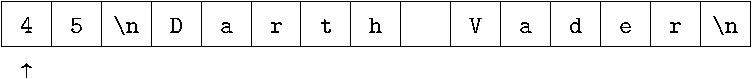
\includegraphics{vader1.pdf}
\end{center}

The up arrow represents the next character to be read.
When you call \java{nextInt}, the \java{Scanner} class will read characters until a non-digit is found.

\begin{center}
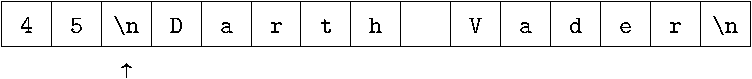
\includegraphics{vader2.pdf}
\end{center}

At this point, \java{nextInt} returns the value \java{45}.
The above example then asks \java{"What is your name? "} and calls \java{nextLine}.
\java{Scanner} will read characters until a newline is found.
Since the next character to be read already is a newline, \java{nextLine} returns the empty string \java{""}.

To solve this problem, you need to add an extra call to \java{nextLine} after you call \java{nextInt}.

\begin{code}
    System.out.print("What is your age? ");
    age = in.nextInt();
    in.nextLine();  // read the newline
    System.out.print("What is your name? ");
    name = in.nextLine();
\end{code}

This technique is common when reading \java{int} or \java{double} values that appear on their own line.
First you read the number, then you read the rest of the line (which is just a newline character).
Note that you do not have to assign the return value of \java{nextLine} to a variable in that case; you can simply ignore it.
